\documentclass[12pt]{article}
\usepackage{setspace, graphicx, fullpage, amssymb, amsmath, epsfig, natbib, array, multirow, hyperref}
\usepackage{amsfonts, bm} 
\usepackage{dcolumn}
\usepackage{subfigure, float} 
\usepackage[margin=1in]{geometry} 
\usepackage{verbatim}
\usepackage{url}
\usepackage{enumerate}
\newcolumntype{d}[1]{D{.}{.}{#1}} 

\begin{document}

\begin{center}
\Large 15 February 2016
\end{center}

\section{Overview}

The main tasks I set out to accomplish over week as per our last meeting were as follows:

\begin{itemize}
	\item Finish testing differences between the ``Summer'' and ``Winter'' model specifications for the Senate to determine what led to changes in results.
	
	\item Conduct tests on specifications of the models which might be meaningfully different in their results.
	
	\item Remake the graphs from last week with \verb|pirate100| replaced by \verb|pfrate100| in the Senate, as well as showing similar graphs for the House.
\end{itemize}

\noindent
William graciously took the time to build an updated version of the Summer algorithm to include the changes we've made which are still in use. This allowed us to turn changes we'd made off and on again so we could see what the meaningful changes were. We found the same changes produced by keeping very lopsided votes in the sorting as were shown last week and choosing between OLS and bias-reduced logit to identify party influence in votes (with OLS sorting more votes as party calls, as predicted). I tested a specification which was set up like the Winter model except for these two aspects on Senate 95 (which produced very different results between the Summer and Winter) against the Summer model and found that each model shared 344 party calls with each only having a single vote as a party call that the other didn't.

While there is good reason to stick with the bias-reduced logit instead of OLS, it remains worth considering whether we should be setting the same threshold for dropping votes in the Senate that we use in the House, given that there are over 4 times as many members of the House than the Senate. So, it means something entirely different when a House vote has 4 members on one side than it does for a Senate vote. For this reason, below I show the differences in results produced by keeping these votes in beyond the vote sorting I showed last week. William hypothesized that the noncalls we were losing were causing us to lose meaningful information about member ideology and that the model as specified was too liberal in removing votes in the Senate. Since testing showed these results to be largely the same between models, I used the sorting from the Winter model to test this, with results reported below. 

I further show the Senate figures with \verb|pfrate100| as the $y$ variable in and the same tables from last week repeated for the House as requested at our last meeting. Rather than do DV/DV plots for the House, I plotted the replication data from Minozzi \& Volden (2013) so we can compare these. It's worth noting that the old method produced less of a drop off for Democrats (though the same or more for Republicans).

\pagebreak



\section{Tables and Figures}

\subsection{Summary Statistics, Senate with Very Lopsided Votes}

% Table created by stargazer v.5.2 by Marek Hlavac, Harvard University. E-mail: hlavac at fas.harvard.edu
% Date and time: Mon, Feb 13, 2017 - 14:41:16
\begin{table}[!htbp] \centering 
	\caption{Main DV and IV Range, Senate with Very Lopsided Votes} 
	\begin{tabular}{@{\extracolsep{5pt}}lccccc} 
		\\[-1.8ex]\hline 
		\hline \\[-1.8ex] 
		Statistic & \multicolumn{1}{c}{N} & \multicolumn{1}{c}{Mean} & \multicolumn{1}{c}{St. Dev.} & \multicolumn{1}{c}{Min} & \multicolumn{1}{c}{Max} \\ 
		\hline \\[-1.8ex] 
		Party Free Ideal Point - All & 1,990 & 0.002 & 1.000 & $-$2.040 & 2.808 \\ 
		pirate100 - All & 1,990 & 82.257 & 11.347 & 12.500 & 100.000 \\ 
		pfrate100 - All & 1,990 & 87.077 & 7.891 & 41.889 & 100.000 \\ 
		Ideological Extremism - All & 1,990 & 0.827 & 0.562 & $-$1.589 & 2.808 \\ 
		\hline
		Party Free Ideal Point - Dems & 1,039 & $-$0.790 & 0.522 & $-$2.040 & 1.589 \\ 
		pirate100 - Dems & 1,039 & 82.664 & 11.033 & 12.500 & 100.000 \\ 
		pfrate100 - Dems & 1,039 & 87.926 & 7.713 & 41.889 & 100.000 \\ 
		Ideological Extremism - Dems & 1,039 & 0.790 & 0.522 & $-$1.589 & 2.040 \\ 
		\hline 
		Party Free Ideal Point - Reps & 951 & 0.867 & 0.600 & $-$1.279 & 2.808 \\ 
		pirate100 - Reps & 951 & 81.813 & 11.671 & 35.897 & 100.000 \\ 
		pfrate100 - Reps & 951 & 86.151 & 7.984 & 52.927 & 100.000 \\ 
		Ideological Extremism - Reps & 951 & 0.867 & 0.600 & $-$1.279 & 2.808 \\
		\hline
		Party Free Ideal Point - Maj & 1,049 & $-$0.057 & 0.901 & $-$1.924 & 2.511 \\ 
		pirate100 - Maj & 1,049 & 83.089 & 10.982 & 35.516 & 100.000 \\ 
		pfrate100 - Maj & 1,049 & 88.131 & 7.484 & 50.772 & 100.000 \\ 
		Ideological Extremism - Maj & 1,049 & 0.737 & 0.521 & $-$1.589 & 2.511 \\ 
		\hline
		Party Free Ideal Point - Min & 843 & 0.074 & 1.106 & $-$2.040 & 2.808 \\ 
		pirate100 - Min & 843 & 80.848 & 11.615 & 12.500 & 100.000 \\ 
		pfrate100 - Min & 843 & 85.266 & 8.219 & 41.889 & 100.000 \\ 
		Ideological Extremism - Min & 843 & 0.924 & 0.611 & $-$1.279 & 2.808 \\ 
		\hline \\[-1.8ex] 
	\end{tabular} 
\end{table} 

\begin{table}[!htbp]
	\begin{center}
		\caption{Bivariate DV IV Regression, Senate with Very Lopsided Votes}
		\begin{tabular}{l c c c c }
			\hline
			& Democrats & Democrats & Republicans & Republicans \\
			\hline
			pfrate100              & $1.17^{***}$   &               & $1.19^{***}$   &               \\
			& $(0.03)$       &               & $(0.03)$       &               \\
			ideological\_extremism &                & $12.78^{***}$ &                & $10.53^{***}$ \\
			&                & $(0.52)$      &                & $(0.53)$      \\
			(Intercept)            & $-20.46^{***}$ & $72.57^{***}$ & $-20.81^{***}$ & $72.68^{***}$ \\
			& $(2.24)$       & $(0.49)$      & $(2.38)$       & $(0.56)$      \\
			\hline
			R$^2$                  & 0.67           & 0.37          & 0.66           & 0.29          \\
			Adj. R$^2$             & 0.67           & 0.37          & 0.66           & 0.29          \\
			Num. obs.              & 1039           & 1039          & 951            & 951           \\
			RMSE                   & 6.32           & 8.79          & 6.77           & 9.82          \\
			\hline
			\multicolumn{5}{l}{\scriptsize{$^{***}p<0.001$, $^{**}p<0.01$, $^*p<0.05$}}
		\end{tabular}
	\end{center}
\end{table}

\begin{table}[!htbp]
	\begin{center}
		\caption{Multivariate DV IV Regression, Senate with Very Lopsided Votes}
		\begin{tabular}{l c c c c }
			\hline
			& Democrats & Republicans & Majority & Minority \\
			\hline
			pfrate100              & $1.087^{***}$   & $1.076^{***}$   & $1.151^{***}$   & $0.991^{***}$ \\
			& $(0.035)$       & $(0.032)$       & $(0.033)$       & $(0.036)$     \\
			ideological\_extremism & $1.861^{***}$   & $2.866^{***}$   & $1.659^{***}$   & $3.043^{***}$ \\
			& $(0.510)$       & $(0.423)$       & $(0.475)$       & $(0.485)$     \\
			(Intercept)            & $-14.388^{***}$ & $-13.365^{***}$ & $-19.562^{***}$ & $-6.464^{*}$  \\
			& $(2.782)$       & $(2.573)$       & $(2.699)$       & $(2.837)$     \\
			\hline
			R$^2$                  & 0.676           & 0.680           & 0.703           & 0.653         \\
			Adj. R$^2$             & 0.676           & 0.679           & 0.703           & 0.652         \\
			Num. obs.              & 1039            & 951             & 1049            & 843           \\
			RMSE                   & 6.282           & 6.614           & 5.989           & 6.851         \\
			\hline
			\multicolumn{5}{l}{\scriptsize{$^{***}p<0.001$, $^{**}p<0.01$, $^*p<0.05$}}
		\end{tabular}
	\end{center}
\end{table}

\pagebreak

\subsection{IV / IV Plots, Senate without Very Lopsided Votes}

\begin{figure}[!htbp]
	\caption{IV IV Plot - Senate Majority and Minority Party Democrats \textit{Note}: The light gray line and dots are for Congress 107.}
	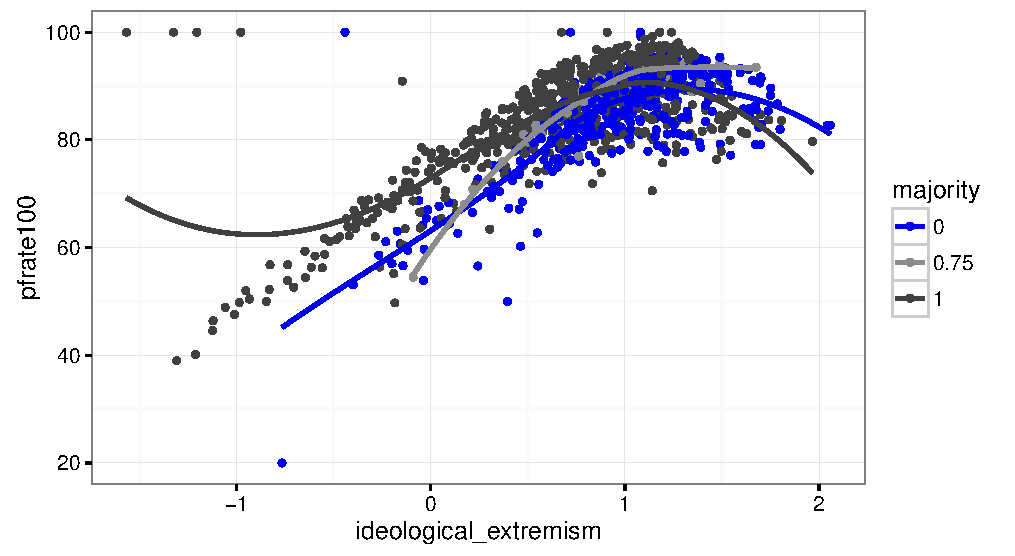
\includegraphics[width = \textwidth]{C:/Users/Ethan/Documents/GitHub/partycalls/plots/senate_p_05_dem_iv_iv_2_majority.pdf}
\end{figure}

\begin{figure}[!htbp]
	\caption{IV IV Plot - Senate Southern and Other Democrats}
	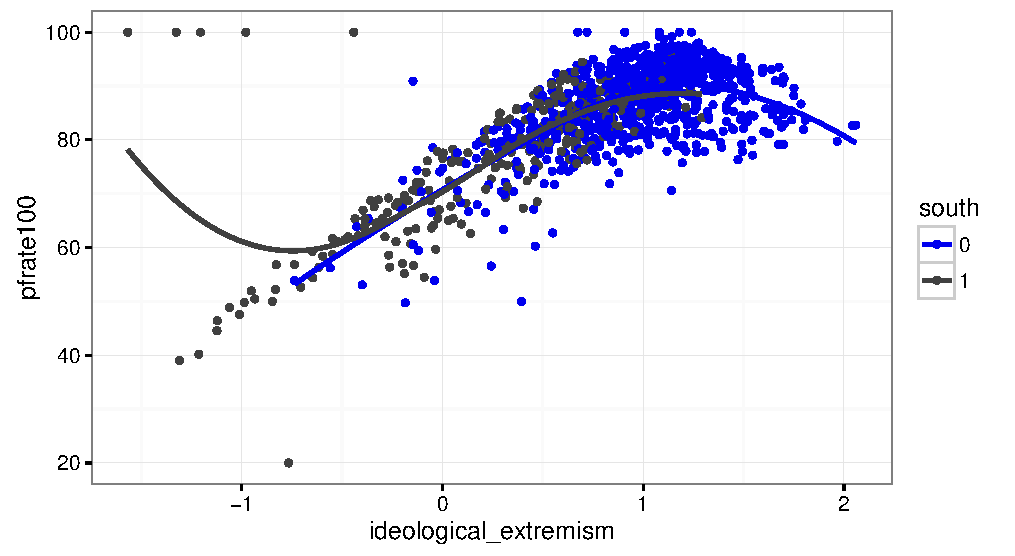
\includegraphics[width = \textwidth]{C:/Users/Ethan/Documents/GitHub/partycalls/plots/senate_p_05_dem_iv_iv_2_south.pdf}
\end{figure}

\begin{figure}[!htbp]
	\caption{IV IV Plot - Senate Majority and Minority Party Republicans \textit{Note}: The light gray line and dots are for Congress 107.}
	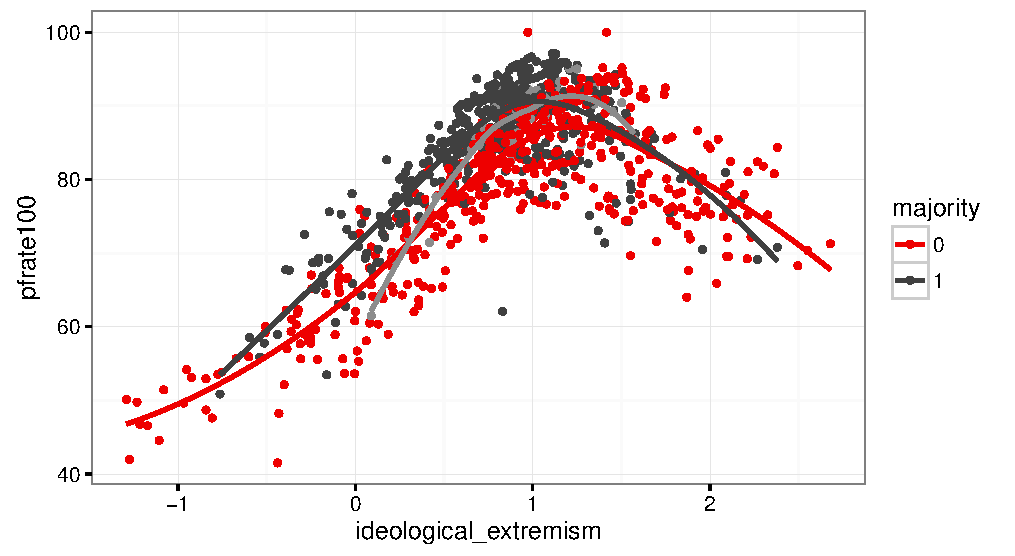
\includegraphics[width = \textwidth]{C:/Users/Ethan/Documents/GitHub/partycalls/plots/senate_p_05_rep_iv_iv_2_majority.pdf}
\end{figure}

\begin{figure}[!htbp]
	\caption{IV IV Plot - Senate Southern and Other Republicans}
	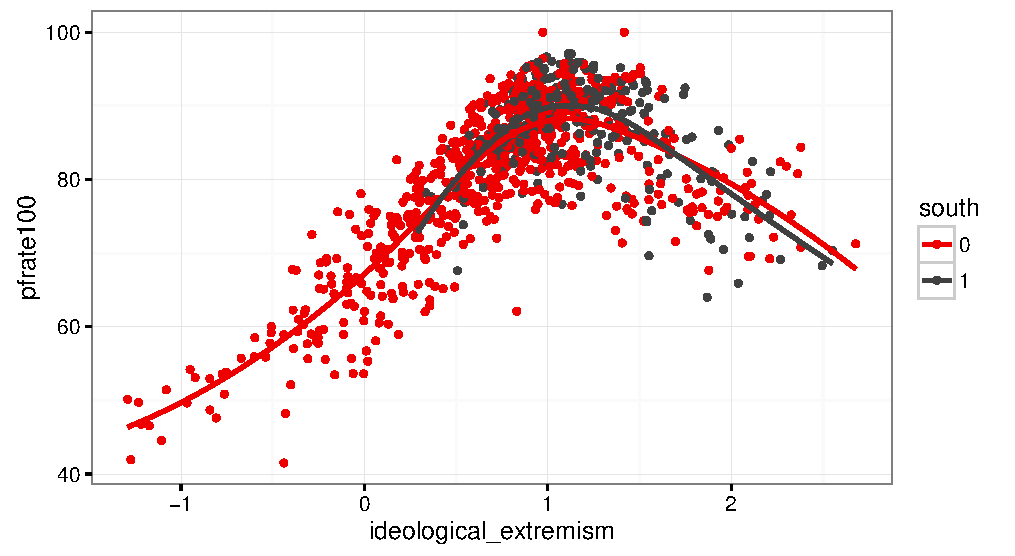
\includegraphics[width = \textwidth]{C:/Users/Ethan/Documents/GitHub/partycalls/plots/senate_p_05_rep_iv_iv_2_south.pdf}
\end{figure}

\begin{figure}[!htbp]
	\caption{IV IV Plot - Gingrich Senators and Other Senate Republicans}
	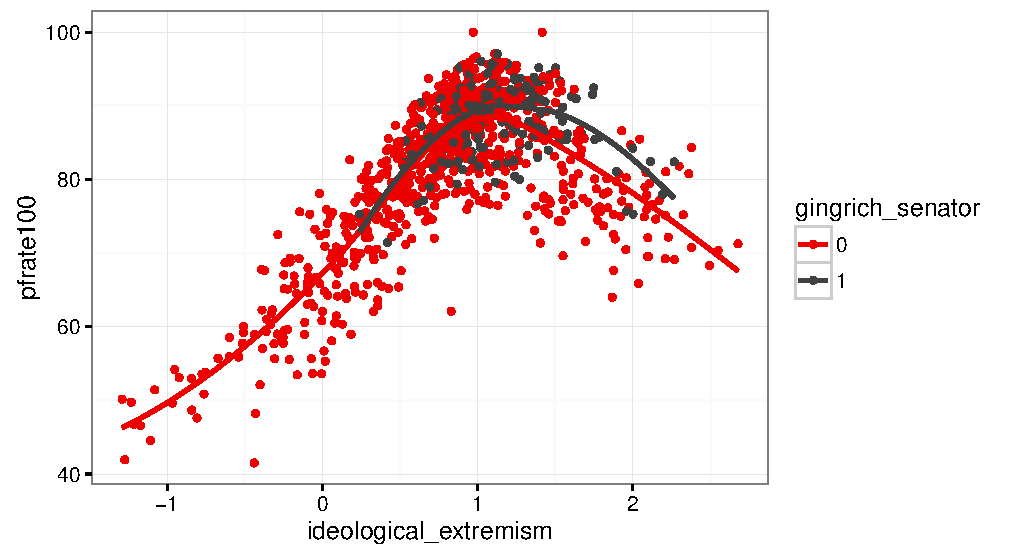
\includegraphics[width = \textwidth]{C:/Users/Ethan/Documents/GitHub/partycalls/plots/senate_p_05_rep_iv_iv_2_gingrich.pdf}
\end{figure}

\subsection{House DV IV Plots and Regressions}

\begin{table}[!htbp]
	\begin{center}
		\caption{Bivariate DV IV Regression, New House}
		\begin{tabular}{l c c c c }
			\hline
			& Democrats & Democrats & Republicans & Republicans \\
			\hline
			pfrate100              & $1.18^{***}$   &               & $0.78^{***}$  &               \\
			& $(0.01)$       &               & $(0.02)$      &               \\
			ideological\_extremism &                & $14.15^{***}$ &               & $10.57^{***}$ \\
			&                & $(0.21)$      &               & $(0.30)$      \\
			(Intercept)            & $-20.61^{***}$ & $72.07^{***}$ & $15.89^{***}$ & $74.36^{***}$ \\
			& $(1.07)$       & $(0.20)$      & $(1.35)$      & $(0.32)$      \\
			\hline
			R$^2$                  & 0.66           & 0.49          & 0.41          & 0.24          \\
			Adj. R$^2$             & 0.66           & 0.49          & 0.41          & 0.24          \\
			Num. obs.              & 4741           & 4742          & 3805          & 3807          \\
			RMSE                   & 7.02           & 8.68          & 8.08          & 9.14          \\
			\hline
			\multicolumn{5}{l}{\scriptsize{$^{***}p<0.001$, $^{**}p<0.01$, $^*p<0.05$}}
		\end{tabular}
	\end{center}
\end{table}

\begin{table}[!htbp]
	\begin{center}
		\caption{Multivariate DV IV Regression, New House}
		\begin{tabular}{l c c c c }
			\hline
			& Democrats & Republicans & Majority & Minority \\
			\hline
			pfrate100              & $0.902^{***}$ & $0.689^{***}$  & $0.777^{***}$ & $0.616^{***}$  \\
			& $(0.015)$     & $(0.014)$      & $(0.015)$     & $(0.015)$      \\
			ideological\_extremism & $6.024^{***}$ & $8.129^{***}$  & $8.080^{***}$ & $8.895^{***}$  \\
			& $(0.205)$     & $(0.241)$      & $(0.216)$     & $(0.233)$      \\
			(Intercept)            & $-0.918$      & $16.652^{***}$ & $9.987^{***}$ & $20.008^{***}$ \\
			& $(1.191)$     & $(1.182)$      & $(1.226)$     & $(1.187)$      \\
			\hline
			R$^2$                  & 0.716         & 0.542          & 0.711         & 0.574          \\
			Adj. R$^2$             & 0.716         & 0.542          & 0.710         & 0.574          \\
			Num. obs.              & 4741          & 3805           & 4903          & 3643           \\
			RMSE                   & 6.457         & 7.097          & 6.331         & 6.938          \\
			\hline
			\multicolumn{5}{l}{\scriptsize{$^{***}p<0.001$, $^{**}p<0.01$, $^*p<0.05$}}
		\end{tabular}
	\end{center}
\end{table}

\begin{table}[!htbp]
	\begin{center}
		\caption{Bivariate DV IV Regression, Old House}
		\begin{tabular}{l c c c c }
			\hline
			& Democrats & Democrats & Republicans & Republicans \\
			\hline
			pfrate100              & $1.14^{***}$   &                & $0.80^{***}$  &               \\
			& $(0.02)$       &                & $(0.02)$      &               \\
			ideological\_extremism &                & $13.71^{***}$  &               & $7.46^{***}$  \\
			&                & $(0.19)$       &               & $(0.30)$      \\
			(Intercept)            & $-14.31^{***}$ & $141.61^{***}$ & $16.72^{***}$ & $40.39^{***}$ \\
			& $(1.41)$       & $(0.83)$       & $(1.47)$      & $(1.75)$      \\
			\hline
			R$^2$                  & 0.54           & 0.56           & 0.40          & 0.17          \\
			Adj. R$^2$             & 0.54           & 0.56           & 0.40          & 0.17          \\
			Num. obs.              & 4059           & 4059           & 3187          & 3187          \\
			RMSE                   & 7.97           & 7.79           & 7.88          & 9.30          \\
			\hline
			\multicolumn{5}{l}{\scriptsize{$^{***}p<0.001$, $^{**}p<0.01$, $^*p<0.05$}}
		\end{tabular}
	\end{center}
\end{table}

\begin{table}[!htbp]
	\begin{center}
		\caption{Multivariate DV IV Regression, Old House}
		\begin{tabular}{l c c c c }
			\hline
			& Democrats & Republicans & Majority & Minority \\
			\hline
			pfrate100              & $0.717^{***}$  & $0.749^{***}$   & $1.033^{***}$  & $0.716^{***}$  \\
			& $(0.016)$      & $(0.016)$       & $(0.014)$      & $(0.020)$      \\
			ideological\_extremism & $9.069^{***}$  & $6.081^{***}$   & $0.798^{***}$  & $-0.385^{***}$ \\
			& $(0.184)$      & $(0.228)$       & $(0.022)$      & $(0.031)$      \\
			(Intercept)            & $60.444^{***}$ & $-14.560^{***}$ & $-4.292^{***}$ & $23.996^{***}$ \\
			& $(1.887)$      & $(1.772)$       & $(1.214)$      & $(1.694)$      \\
			\hline
			R$^2$                  & 0.712          & 0.511           & 0.681          & 0.358          \\
			Adj. R$^2$             & 0.711          & 0.511           & 0.681          & 0.357          \\
			Num. obs.              & 4059           & 3187            & 4184           & 3062           \\
			RMSE                   & 6.311          & 7.126           & 6.535          & 8.332          \\
			\hline
			\multicolumn{5}{l}{\scriptsize{$^{***}p<0.001$, $^{**}p<0.01$, $^*p<0.05$}}
		\end{tabular}
	\end{center}
\end{table}


\begin{figure}[ht]
	\caption{Main DV and Ideological Extremism - Southern and Other House Democrats}
	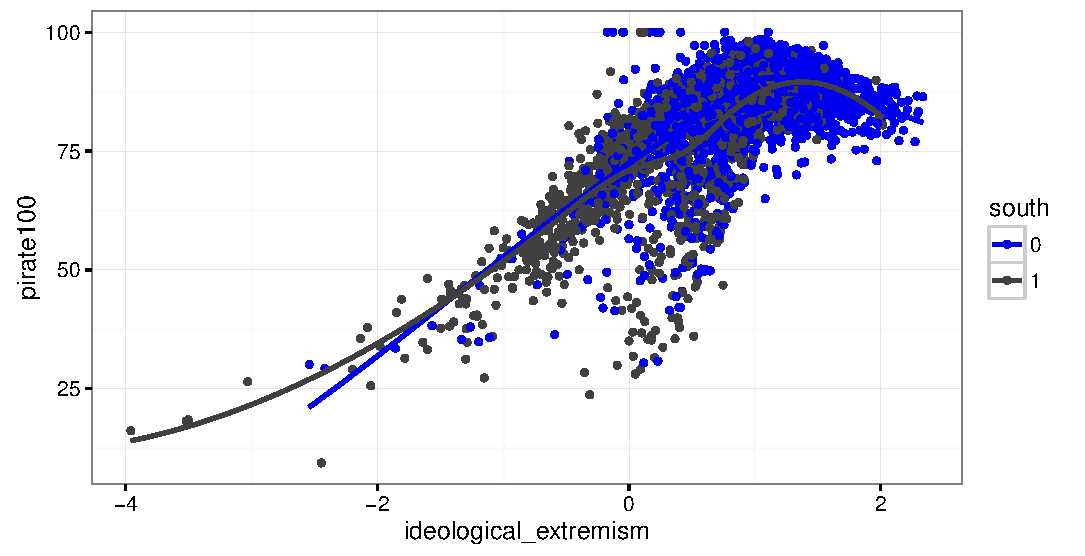
\includegraphics[width = \textwidth]{C:/Users/Ethan/Documents/GitHub/partycalls/plots/house_dem_iv-dv_2_south.pdf}
\end{figure}

\begin{figure}[ht]
	\caption{Main DV and Ideological Extremism - Majority and Minority House Democrats}
	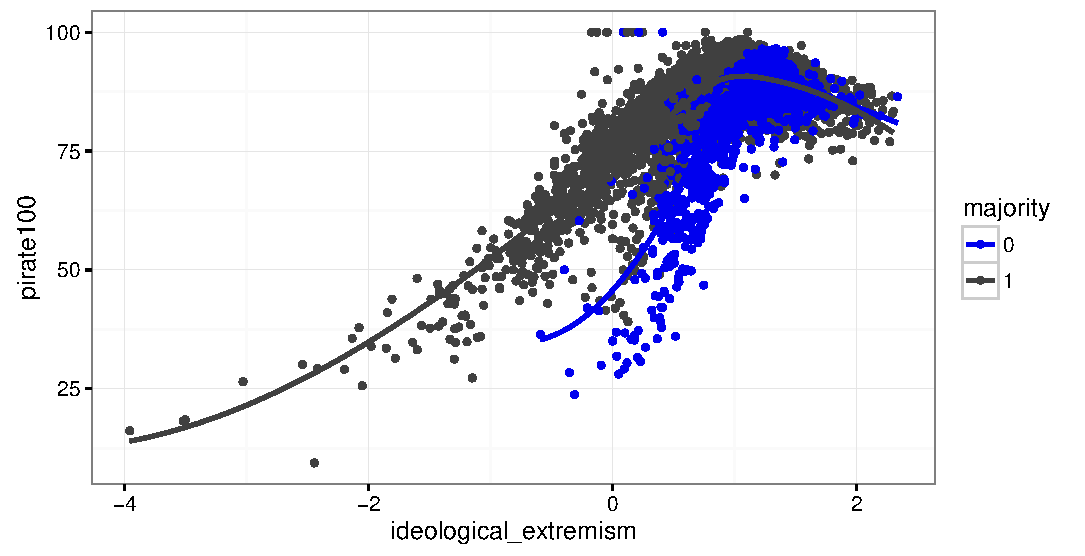
\includegraphics[width = \textwidth]{C:/Users/Ethan/Documents/GitHub/partycalls/plots/house_dem_iv-dv_2_majority.pdf}
\end{figure}

\begin{figure}[ht]
	\caption{Main DV and Ideological Extremism - Southern and Other House Republicans}
	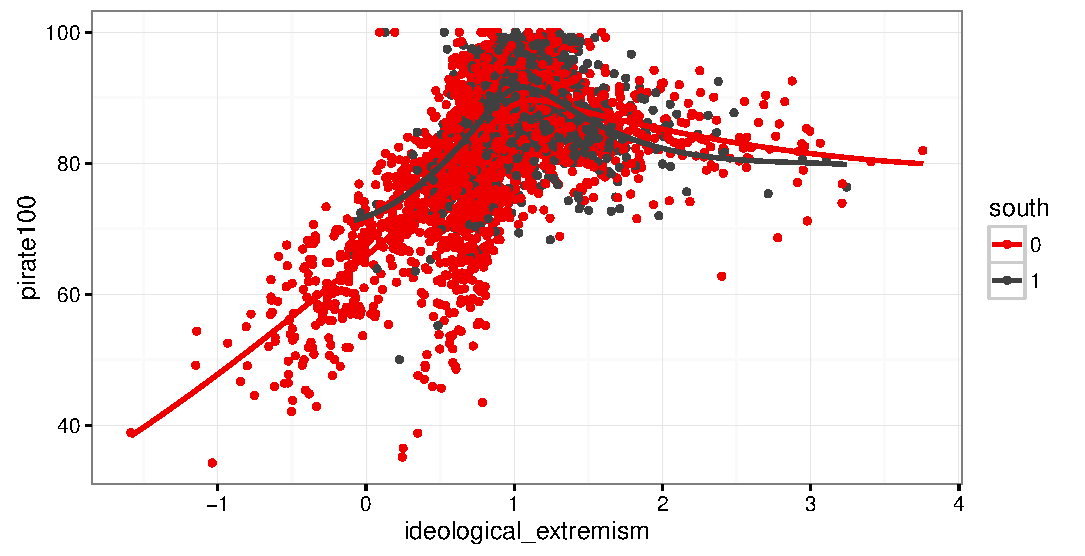
\includegraphics[width = \textwidth]{C:/Users/Ethan/Documents/GitHub/partycalls/plots/house_rep_iv-dv_2_south.pdf}
\end{figure}

\begin{figure}[ht]
	\caption{Main DV and Ideological Extremism - Majority and Minority House Republicans}
	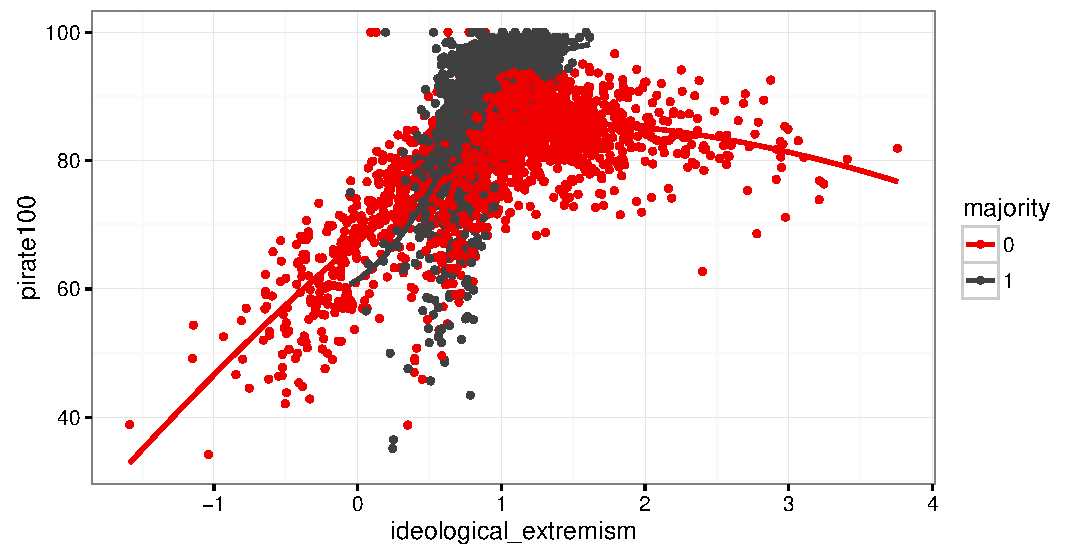
\includegraphics[width = \textwidth]{C:/Users/Ethan/Documents/GitHub/partycalls/plots/house_rep_iv-dv_2_majority.pdf}
\end{figure}



\begin{figure}[ht]
	\caption{Main DV and Ideological Extremism - Southern and Other House Democrats, Minozzi \& Volden 2013}
	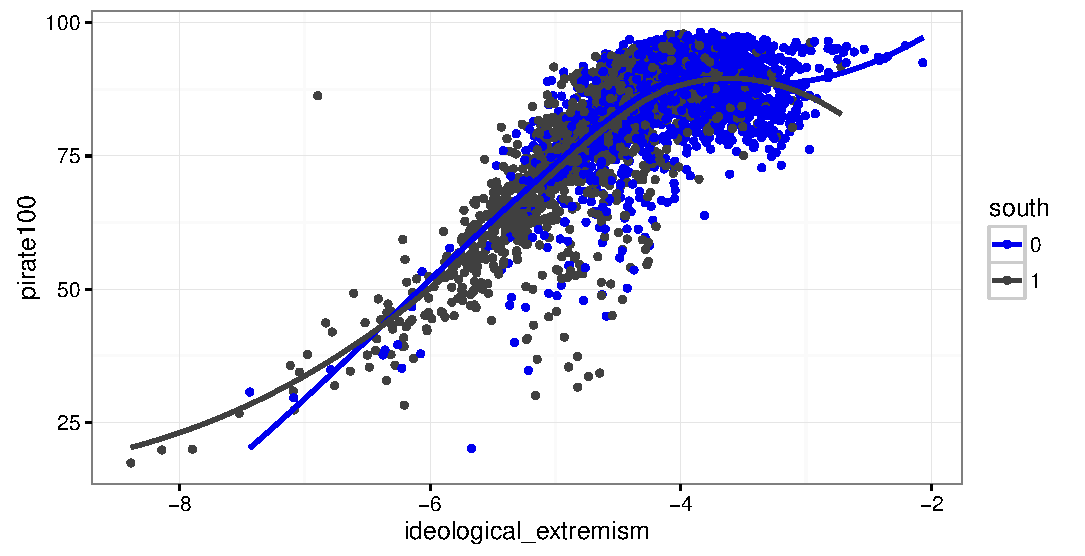
\includegraphics[width = \textwidth]{C:/Users/Ethan/Documents/GitHub/partycalls/plots/house_old_dem_iv-dv_2_south.pdf}
\end{figure}

\begin{figure}[ht]
	\caption{Main DV and Ideological Extremism - Majority and Minority House Democrats, Minozzi \& Volden 2013}
	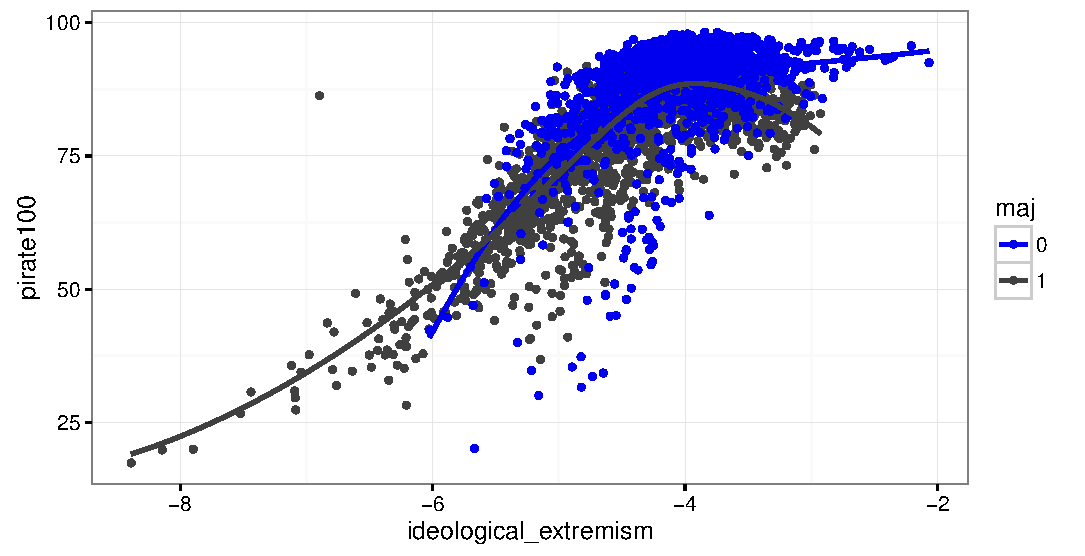
\includegraphics[width = \textwidth]{C:/Users/Ethan/Documents/GitHub/partycalls/plots/house_old_dem_iv-dv_2_maj.pdf}
\end{figure}

\begin{figure}[ht]
	\caption{Main DV and Ideological Extremism - Southern and Other House Republicans, Minozzi \& Volden 2013}
	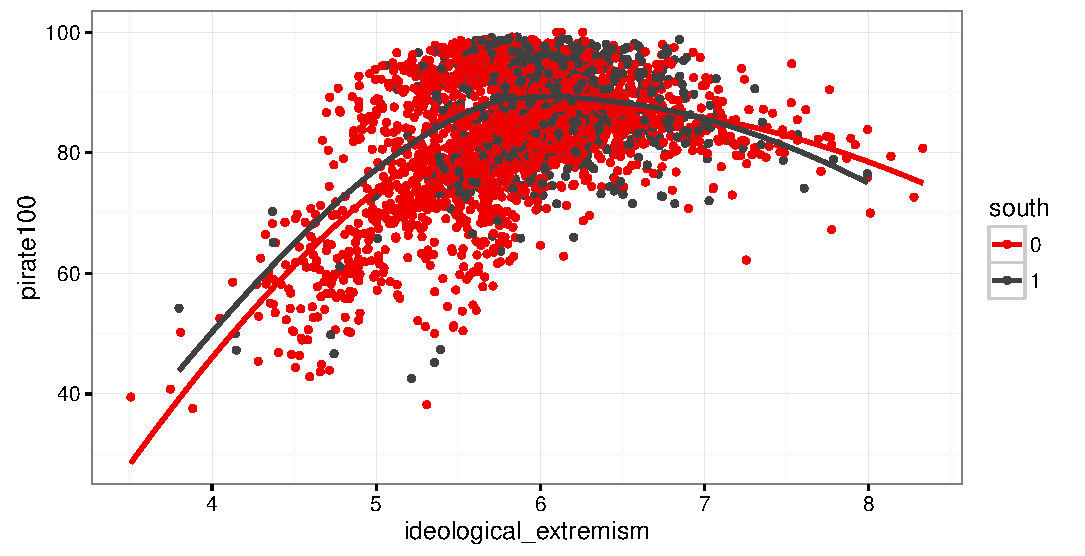
\includegraphics[width = \textwidth]{C:/Users/Ethan/Documents/GitHub/partycalls/plots/house_old_rep_iv-dv_2_south.pdf}
\end{figure}

\begin{figure}[ht]
	\caption{Main DV and Ideological Extremism - Majority and Minority House Republicans, Minozzi \& Volden 2013}
	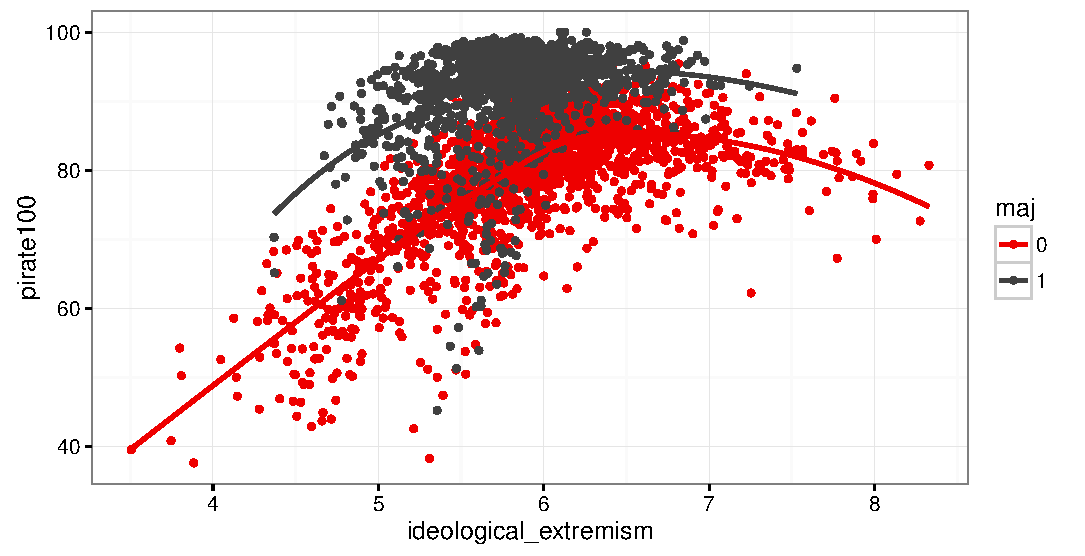
\includegraphics[width = \textwidth]{C:/Users/Ethan/Documents/GitHub/partycalls/plots/house_old_rep_iv-dv_2_maj.pdf}
\end{figure}











\end{document}